\chapter{TINJAUAN PUSTAKA}

\section{Landasan Teori}

\subsection{Traffic Engineering}
\textit{Traffic Engineering} (TE) adalah disiplin rekayasa jaringan yang berfokus pada pengukuran, pemodelan, karakterisasi, dan kontrol lalu lintas internet untuk mengoptimalkan kinerja jaringan. Tujuan utama TE adalah meminimalkan kongesti dan meningkatkan pemanfaatan sumber daya melalui penyeimbangan beban trafik (\textit{load balancing}) \cite{marouani2024}.

TE modern membutuhkan kemampuan untuk menangani pola trafik yang dinamis dan beragam, di mana pendekatan konvensional berbasis algoritma statis seperti jalur terpendek (Dijkstra) seringkali tidak mampu beradaptasi dengan kondisi jaringan yang berubah secara real-time. Oleh karena itu, pendekatan berbasis kecerdasan buatan semakin diperlukan untuk melakukan optimasi distribusi trafik secara adaptif dan efisien.

\begin{figure}[H]
    \centering
    \includegraphics[width=0.8\textwidth]{images/te.png}
    \caption{Ilustrasi Traffic Engineering dalam Jaringan}
    \label{fig:traffic_engineering}
\end{figure}

\subsection{Jaringan Layer 2 dan VLAN}
Jaringan Layer 2 beroperasi pada lapisan \textit{Data Link} dalam model OSI, di mana perangkat \textit{switch} mengirimkan frame berdasarkan alamat MAC\@. Teknologi VLAN (\textit{Virtual Local Area Network}) memungkinkan segmentasi jaringan secara logis dalam satu infrastruktur fisik, meningkatkan keamanan dan efisiensi manajemen jaringan. Segmentasi VLAN terbukti dapat meningkatkan performa jaringan dengan membagi \textit{broadcast domain} yang besar menjadi domain-domain yang lebih kecil dan terkelola \cite{warse2025vlan}.

Pada lingkungan ISP yang menggunakan infrastruktur \textit{switching} Layer 2 dengan VLAN, penerapan Traffic Engineering menghadapi tantangan khusus. Mekanisme \textit{Spanning Tree Protocol} (STP) pada Layer 2 cenderung memblokir jalur redundan untuk mencegah \textit{looping}, yang mengakibatkan tautan cadangan tidak termanfaatkan (\textit{underutilized}) \cite{rashid2024performance, aruba2025campus}. Meskipun varian yang lebih modern seperti \textit{Rapid Spanning Tree Protocol} (RSTP) menawarkan konvergensi yang lebih cepat, kondisi ini tetap membuat optimasi jalur menjadi lebih kompleks dibandingkan jaringan IP tradisional (Layer 3) \cite{ahmad2020intervlan}. Oleh karena itu, diperlukan pendekatan cerdas untuk memprediksi kegagalan dan mendistribusikan trafik secara dinamis tanpa melanggar topologi logis Layer 2 \cite{alhachem2025}.

\begin{figure}[H]
    \centering
    % \includegraphics[width=0.8\textwidth]{images/layer2_vlan.png}
    \caption{Arsitektur Jaringan Layer 2 dengan VLAN}
    \label{fig:layer2_vlan}
\end{figure}

\subsection{Kriteria Evaluasi Kualitas Jalur}

Dalam penelitian ini, kualitas jalur jaringan dievaluasi berdasarkan dua kategori utama kriteria: kriteria tingkat node dan kriteria tingkat edge. Pendekatan dual-level ini memastikan evaluasi yang komprehensif dengan mempertimbangkan baik kemampuan perangkat maupun kualitas koneksi \cite{joint_node_edge_optimization, holistic_network_metrics}.

\subsubsection{Kriteria Tingkat Node}

Kriteria tingkat node mengevaluasi kapasitas dan kondisi operasional dari perangkat jaringan (switch/router) yang dilalui oleh sebuah jalur. Berdasarkan literatur resource-aware routing \cite{resource_aware_sdn, node_capacity_routing}, terdapat 6 kriteria yang dipilih:

\begin{enumerate}
    \item \textbf{CPU Score}: Normalized CPU utilization yang menunjukkan ketersediaan processing power \cite{cpu_aware_routing}.
    \item \textbf{RAM Score}: Normalized memory availability untuk buffering dan state management \cite{node_capacity_routing}.
    \item \textbf{Traffic In}: Volume trafik masuk yang sedang ditangani node \cite{utilization_based_te}.
    \item \textbf{Traffic Out}: Volume trafik keluar yang sedang ditangani node \cite{adaptive_utilization_routing}.
    \item \textbf{Utilization Score}: Aggregate interface utilization yang menunjukkan seberapa sibuk node dalam menangani trafik secara keseluruhan \cite{interface_speed_impact}.
    \item \textbf{Status Score}: Binary indicator operational status (up/down) yang sangat penting untuk failure-aware routing \cite{failure_aware_te}.
\end{enumerate}

Skor komposit node dihitung sebagai weighted sum:
\begin{equation}
    S_{node} = \sum_{i=1}^{6} w_i^{node} \cdot f_i^{node}
\end{equation}

\noindent dimana $w_i^{node}$ adalah bobot kriteria yang diperoleh dari AHP dan $f_i^{node}$ adalah nilai kriteria yang telah dinormalisasi.

\subsubsection{Kriteria Tingkat Edge}

Kriteria tingkat edge mengevaluasi karakteristik koneksi fisik atau logis antar perangkat. Mengikuti framework multi-constraint routing \cite{te_multiconstraint}, kriteria yang dipilih meliputi:

\begin{enumerate}
    \item \textbf{Optical Link Quality Score}: Kualitas sinyal optik (OSNR, dBm) pada fiber optic infrastructure \cite{optical_signal_quality}.
    \item \textbf{Error Rate Score}: Inverse dari Bit Error Rate (BER) atau Packet Error Rate (PER) \cite{ber_monitoring}.
    \item \textbf{Packet Loss Score}: Persentase paket yang hilang atau dropped selama transmisi \cite{packet_loss_detection}.
    \item \textbf{Bandwidth Utilization}: Rata-rata utilisasi bandwidth pada kedua arah link (bidirectional average) \cite{bandwidth_aware_te}.
    \item \textbf{Interface Speed}: Kapasitas maksimum interface yang menentukan throughput ceiling \cite{interface_speed_impact}.
    \item \textbf{Distance}: Jarak fisik atau logis yang mempengaruhi propagation delay \cite{geographic_routing}.
    \item \textbf{Status}: Link operational state (up/down) \cite{link_state_routing}.
\end{enumerate}

Skor komposit edge dihitung sebagai:
\begin{equation}
    S_{edge} = \sum_{j=1}^{7} w_j^{edge} \cdot g_j^{edge}
\end{equation}

\noindent dimana terdapat 7 kriteria edge yang digunakan dalam perhitungan bobot.

\paragraph{Perbedaan Optical Quality, Error Rate, dan Packet Loss}

Ketiga metrik ini saling melengkapi dalam mengevaluasi kualitas koneksi pada layer yang berbeda:

\begin{enumerate}
    \item \textbf{Optical Link Quality} (Physical Layer): Mengukur kualitas sinyal cahaya pada fiber optic sebelum proses decoding. Parameter seperti OSNR (Optical Signal-to-Noise Ratio), received optical power (dBm), Q-factor, dan chromatic dispersion mengindikasikan seberapa baik sinyal optik dapat dibedakan dari noise \cite{optical_signal_quality, osnr_monitoring}. Degradasi optical quality dapat disebabkan oleh attenuasi fiber, dispersion, atau interferensi optik.

    \item \textbf{Error Rate} (Data Link Layer): Mengukur tingkat kesalahan bit atau paket setelah proses photodetection, analog-to-digital conversion, dan forward error correction (FEC). BER atau PER menunjukkan berapa banyak bit/paket yang corrupt setelah decoding \cite{ber_per_optical, ber_monitoring}. Bahkan dengan optical quality yang baik, error rate bisa tinggi jika ada masalah pada transceiver atau proses decoding.

    \item \textbf{Packet Loss Rate} (Network Layer): Mengukur paket yang hilang atau di-drop karena congestion, buffer overflow, atau TTL expiry, bukan karena corruption \cite{packet_loss_detection}. Packet loss dapat terjadi meskipun optical quality baik dan error rate rendah, terutama saat terjadi congestion pada switch/router.
\end{enumerate}

Kombinasi ketiga metrik ini memberikan gambaran holistik tentang health dari sebuah link, dari physical layer hingga network layer \cite{holistic_network_metrics}. Integrasi multiple edge metrics ini mengikuti paradigma multi-criteria path selection yang telah terbukti efektif dalam traffic engineering modern \cite{routing_multiple_optimality, madm_heuristic_routing, te_multiconstraint, sdn_multiconstraint_routing}.

Pendekatan weighted composite scoring yang mengintegrasikan kriteria node dan edge ini telah terbukti efektif dalam various QoS routing scenarios \cite{qos_composite_metric, weighted_composite_routing, madm_heuristic_routing, routing_multiple_optimality}.


\subsection{Analytic Hierarchy Process (AHP)}

\textit{Analytic Hierarchy Process} (AHP) adalah metode pengambilan keputusan multikriteria yang dikembangkan oleh Thomas L. Saaty pada tahun 1970 \cite{saaty2008}. AHP dirancang untuk menangani masalah kompleks yang melibatkan berbagai kriteria dengan tingkat kepentingan yang berbeda-beda, dimana setiap alternatif memiliki preferensi yang bervariasi menurut masing-masing kriteria yang digunakan.

Dalam konteks penelitian ini, AHP berperan krusial sebagai metode untuk \textbf{menentukan bobot prioritas fitur} yang valid berdasarkan preferensi pakar. Bobot yang dihasilkan AHP ($\mathbf{w}$) kemudian diintegrasikan ke dalam mekanisme \textit{rule-based scoring} untuk menghasilkan label kualitas jalur ($Q_{path}$) sebagai target pelatihan model GAT. Penggunaan AHP memastikan bahwa perhitungan skor matematis selaras dengan intuisi operasional dari pakar jaringan PT Lare Osing Ndo \cite{khan2020}.

\subsubsection{Prinsip Dasar AHP}

AHP dibangun di atas tiga prinsip fundamental yang menjamin validitas hasil keputusan:

\begin{enumerate}
    \item \textbf{Decomposition (Dekomposisi)}: Memecah masalah kompleks menjadi struktur hierarki yang terdiri dari tujuan, kriteria, dan alternatif yang lebih sederhana dan terukur.

    \item \textbf{Comparative Judgement (Penilaian Komparatif)}: Melakukan perbandingan berpasangan (\textit{pairwise comparison}) antar elemen pada level hierarki yang sama untuk menentukan tingkat kepentingan relatif.

    \item \textbf{Logical Consistency (Konsistensi Logis)}: Memastikan bahwa penilaian yang diberikan bersifat konsisten dan dapat diandalkan melalui pengujian rasio konsistensi.
\end{enumerate}

\subsubsection{Struktur Hierarki AHP}

Struktur hierarki AHP disusun untuk memodelkan preferensi manajemen jaringan ke dalam bentuk bobot kuantitatif. Hasil akhir dari hierarki ini bukanlah pemilihan jalur secara langsung, melainkan seperangkat vektor bobot (\textit{weight vectors}) yang akan digunakan untuk menyusun \textit{ground truth} pada pelatihan model GAT.

Struktur hierarki terdiri dari tiga level sebagai berikut:

\begin{enumerate}
    \item \textbf{Level 1 (Tujuan Utama)}: Menentukan bobot prioritas (\textit{Priority Weights}) dari setiap parameter penentu kualitas jalur.

    \item \textbf{Level 2 (Kategori Kriteria)}: Pengelompokan parameter berdasarkan letaknya dalam struktur graf jaringan:
    \begin{itemize}
        \item \textbf{Kriteria Node}: Parameter yang mengukur kinerja perangkat (\textit{switch}).
        \item \textbf{Kriteria Edge}: Parameter yang mengukur kualitas tautan (\textit{link}).
    \end{itemize}

    \item \textbf{Level 3 (Sub-Kriteria/Indikator)}: Parameter spesifik yang akan diberi bobot:
    \begin{itemize}
        \item \textbf{Sub-Kriteria Node (5 Parameter):}
        \begin{enumerate}
            \item \textbf{CPU Score}: Bobot kepentingan untuk ketersediaan CPU.
            \item \textbf{RAM Score}: Bobot kepentingan untuk ketersediaan memori.
            \item \textbf{Traffic Score}: Bobot kepentingan untuk volume trafik.
            \item \textbf{Utilization Score}: Bobot kepentingan untuk kesibukan interface.
            \item \textbf{Status Score}: Bobot kepentingan untuk status hidup/mati perangkat.
        \end{enumerate}

        \item \textbf{Sub-Kriteria Edge (7 Parameter):}
        \begin{enumerate}
            \item \textbf{Optical Link Quality Score}: Bobot kepentingan kualitas fisik optik.
            \item \textbf{Error Rate Score}: Bobot kepentingan minimnya error transmisi.
            \item \textbf{Packet Loss Score}: Bobot kepentingan reliabilitas pengiriman paket.
            \item \textbf{Bandwidth Utilization}: Bobot kepentingan ketersediaan bandwidth.
            \item \textbf{Interface Speed}: Bobot kepentingan kapasitas maksimum link.
            \item \textbf{Distance}: Bobot kepentingan jarak fisik/logis.
            \item \textbf{Link Status}: Bobot kepentingan status hidup/mati link.
        \end{enumerate}
    \end{itemize}
\end{enumerate}

Output dari proses hierarki ini adalah vektor bobot $\mathbf{w}_{node}$ dan $\mathbf{w}_{edge}$ yang kemudian diaplikasikan dalam persamaan komposit untuk menghasilkan label kualitas jalur ($Q_{path}$) sebagai target pembelajaran model GAT.

\begin{figure}[H]
    \centering
    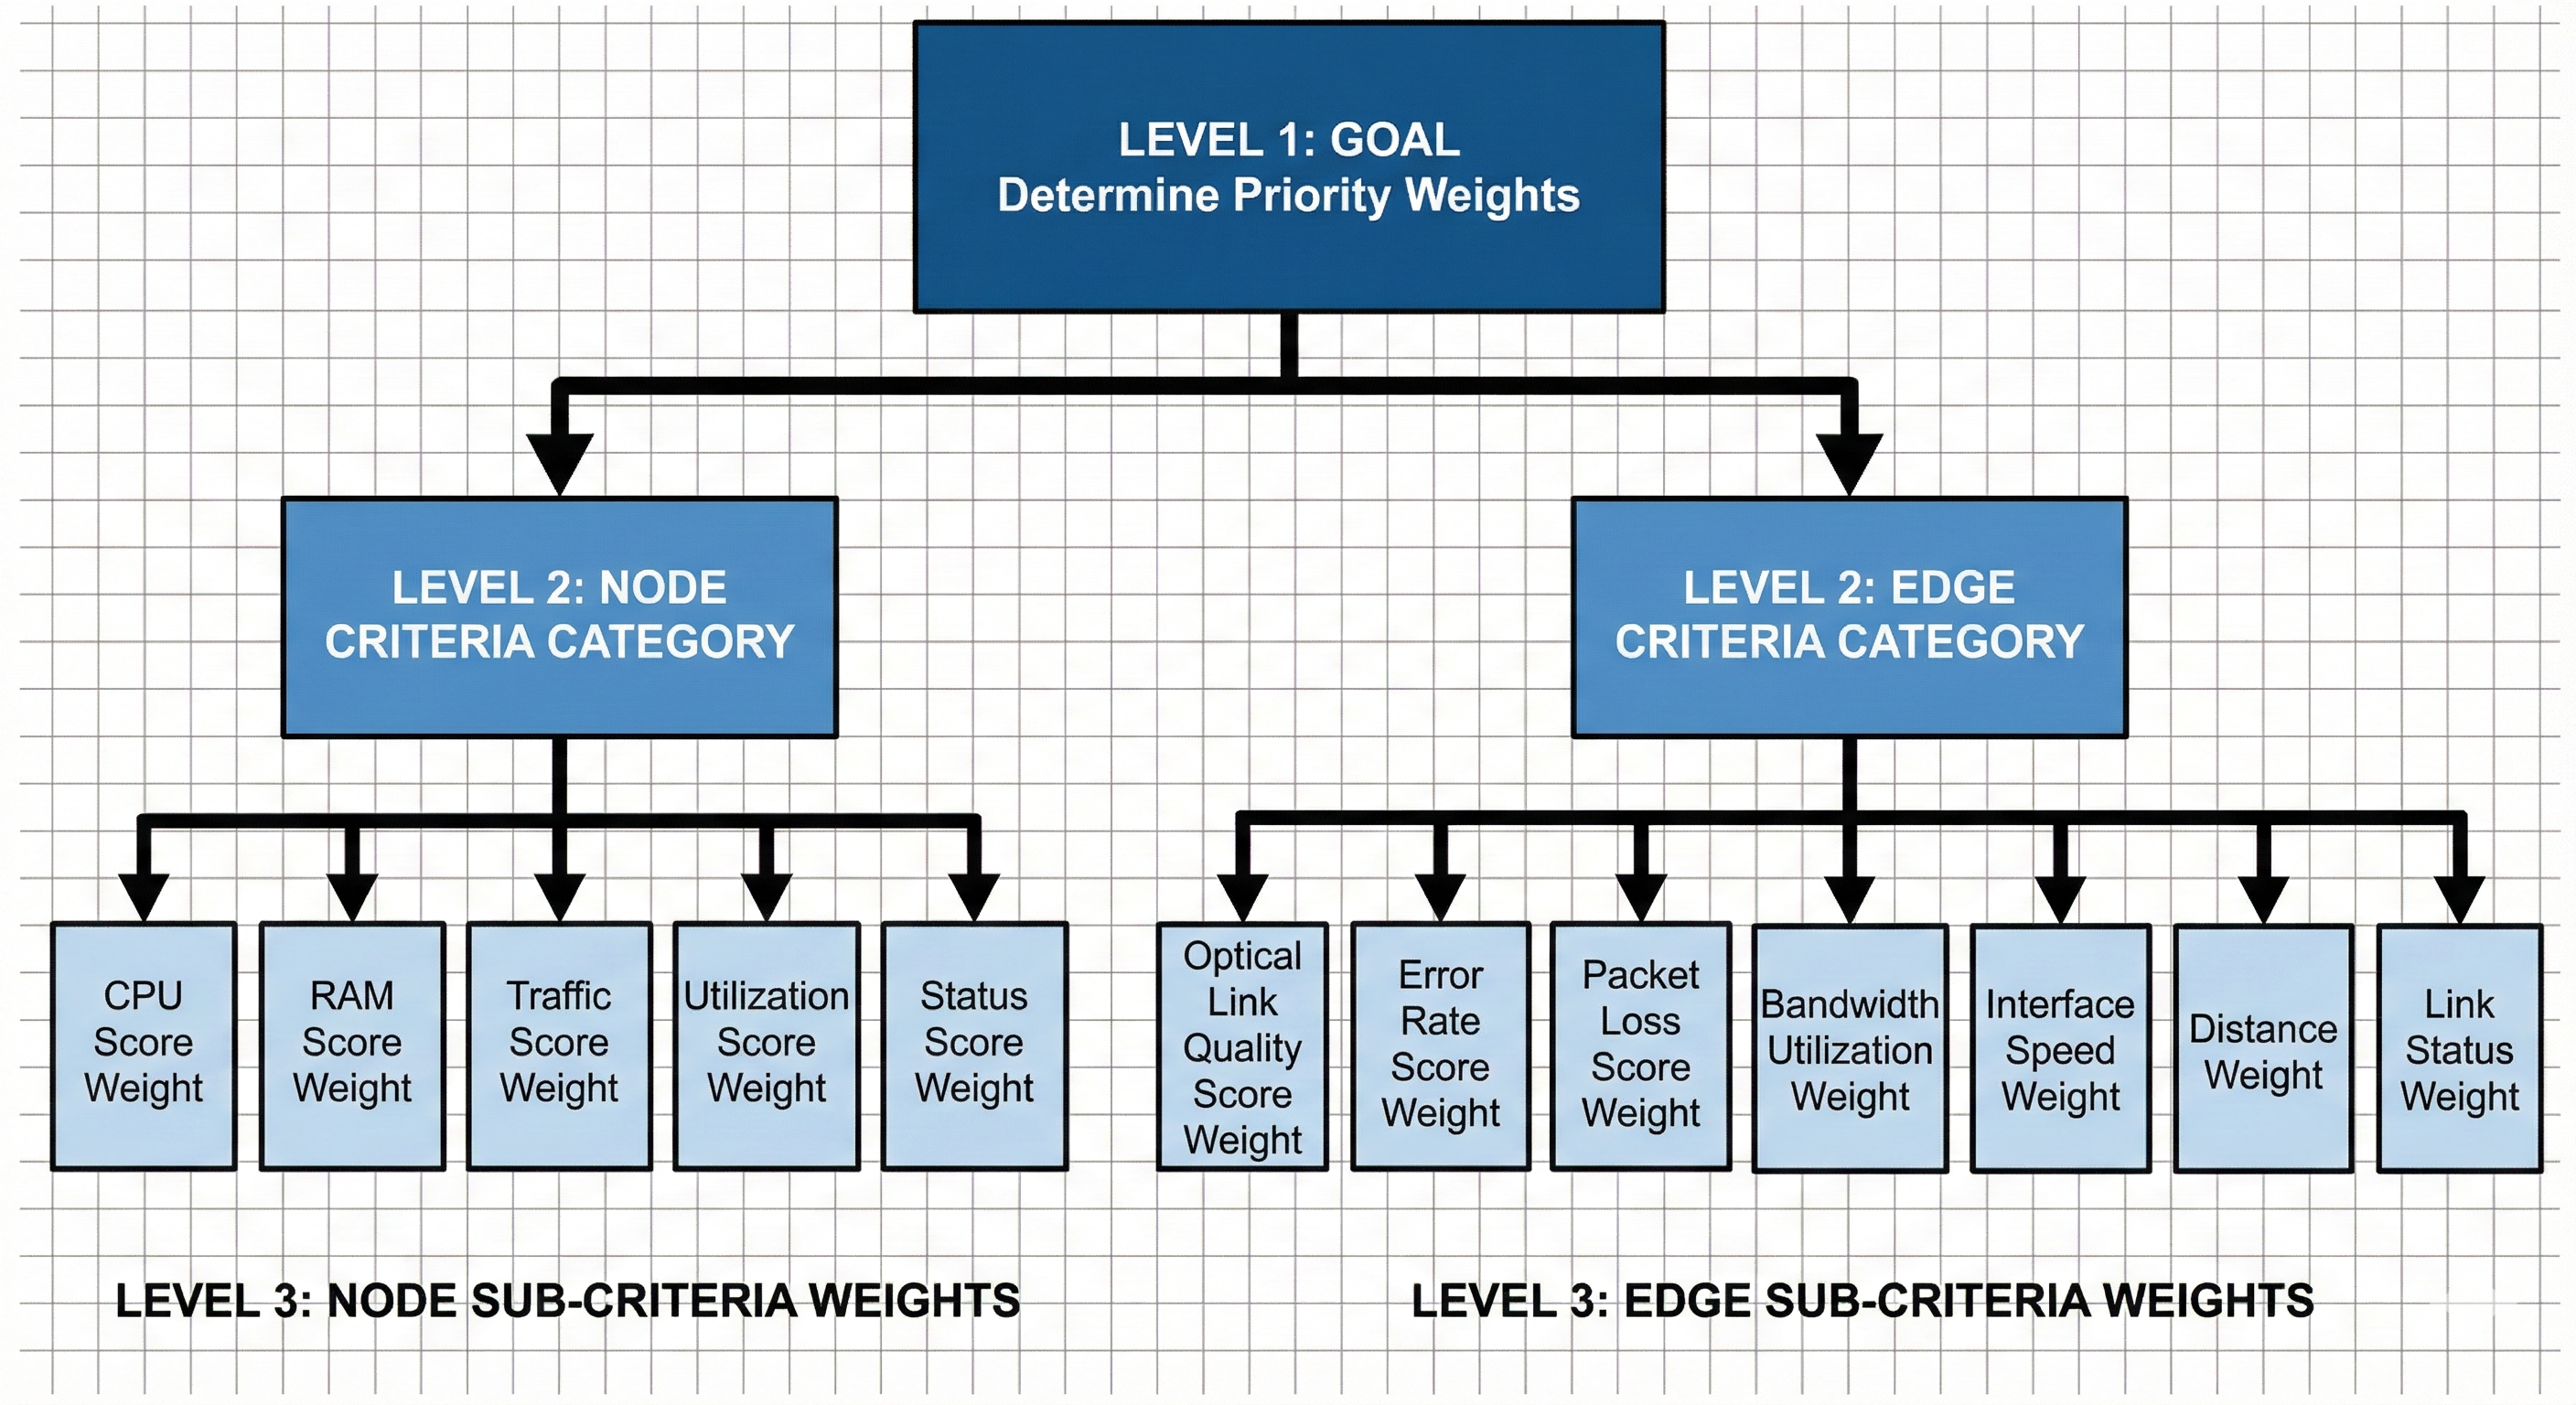
\includegraphics[width=0.9\textwidth]{images/hirarki.png}
    \caption{Struktur Hierarki AHP untuk Penentuan Bobot Parameter}
    \label{fig:ahp_hierarchy}
\end{figure}

\subsubsection{Tahapan Metode AHP}

Implementasi AHP dalam penelitian ini mengikuti lima tahapan sistematis yang dijelaskan sebagai berikut:

\paragraph{1. Penyusunan Matriks Perbandingan Berpasangan}

Tahap pertama adalah membuat matriks perbandingan berpasangan untuk kriteria-kriteria yang telah ditentukan. Setiap pasangan kriteria dibandingkan untuk menentukan tingkat kepentingan relatifnya berdasarkan skala Saaty 1-9.

Matriks perbandingan berpasangan dapat dinyatakan sebagai:

\begin{equation}
    \mathbf{A} = \begin{bmatrix}
        1 & a_{12} & a_{13} & \cdots & a_{1n} \\
        1/a_{12} & 1 & a_{23} & \cdots & a_{2n} \\
        1/a_{13} & 1/a_{23} & 1 & \cdots & a_{3n} \\
        \vdots & \vdots & \vdots & \ddots & \vdots \\
        1/a_{1n} & 1/a_{2n} & 1/a_{3n} & \cdots & 1
    \end{bmatrix}
\end{equation}

\noindent
Dengan:

\begin{tabular}{ll}
$\mathbf{A}$ & = matriks perbandingan berpasangan berukuran $n \times n$ \\
$a_{ij}$ & = tingkat kepentingan kriteria $i$ terhadap kriteria $j$ \\
$n$ & = jumlah kriteria yang dibandingkan
\end{tabular}

\noindent
Matriks ini bersifat resiprokal, yang berarti:

\begin{equation}
    a_{ji} = \frac{1}{a_{ij}}
\end{equation}

\noindent
Dengan:

\begin{tabular}{ll}
$a_{ji}$ & = tingkat kepentingan kriteria $j$ terhadap kriteria $i$
\end{tabular}

\noindent
Sebagai contoh, jika optical link quality dinilai 3 kali lebih penting dari distance, maka:

\begin{equation}
    a_{optical,distance} = 3 \quad \text{dan} \quad a_{distance,optical} = \frac{1}{3}
\end{equation}

\noindent
Dengan:

\begin{tabular}{ll}
$a_{optical,distance}$ & = tingkat kepentingan optical link quality terhadap distance \\
$a_{distance,optical}$ & = tingkat kepentingan distance terhadap optical link quality
\end{tabular}

\noindent
Skala perbandingan yang digunakan mengikuti standar Saaty seperti ditunjukkan pada Tabel \ref{tab:saaty_scale}.

\begin{table}[H]
\centering
\caption{Skala Perbandingan Berpasangan Saaty}
\label{tab:saaty_scale}
\begin{tabular}{|c|l|}
\hline
\textbf{Nilai} & \textbf{Interpretasi} \\
\hline
1 & Kedua elemen sama pentingnya \\
3 & Elemen pertama sedikit lebih penting dari elemen kedua \\
5 & Elemen pertama lebih penting dari elemen kedua \\
7 & Elemen pertama sangat lebih penting dari elemen kedua \\
9 & Elemen pertama mutlak lebih penting dari elemen kedua \\
2, 4, 6, 8 & Nilai antara untuk penilaian yang bersifat kompromistis \\
\hline
\end{tabular}
\end{table}

\paragraph{2. Normalisasi Matriks Perbandingan}

Setelah matriks perbandingan disusun, langkah selanjutnya adalah melakukan normalisasi. Pertama, hitung total nilai setiap kolom:

\begin{equation}
    T_j = \sum_{i=1}^{n} a_{ij}
\end{equation}

\noindent
Dengan:

\begin{tabular}{ll}
$T_j$ & = total nilai pada kolom ke-$j$ \\
$a_{ij}$ & = elemen matriks pada baris ke-$i$ dan kolom ke-$j$ \\
$n$ & = jumlah kriteria yang dibandingkan \\
$i$ & = indeks baris ($i = 1, 2, \ldots, n$)
\end{tabular}

\noindent
Kemudian, setiap elemen matriks dibagi dengan total kolomnya untuk mendapatkan matriks ternormalisasi:

\begin{equation}
    n_{ij} = \frac{a_{ij}}{T_j}
\end{equation}

\noindent
Dengan:

\begin{tabular}{ll}
$n_{ij}$ & = elemen ternormalisasi pada baris $i$ dan kolom $j$ \\
$a_{ij}$ & = elemen matriks asli pada baris $i$ dan kolom $j$ \\
$T_j$ & = total nilai pada kolom ke-$j$
\end{tabular}

\paragraph{3. Perhitungan Vektor Prioritas dan Bobot}

Dari matriks ternormalisasi, vektor prioritas (\textit{Priority Vector}, PV) dihitung dengan menjumlahkan nilai-nilai dalam setiap baris:

\begin{equation}
    PV_i = \sum_{j=1}^{n} n_{ij}
\end{equation}

\noindent
Dengan:

\begin{tabular}{ll}
$PV_i$ & = vektor prioritas untuk kriteria ke-$i$ \\
$n_{ij}$ & = elemen ternormalisasi pada baris $i$ dan kolom $j$ \\
$n$ & = jumlah total kriteria yang dibandingkan \\
$j$ & = indeks kolom ($j = 1, 2, \ldots, n$)
\end{tabular}

\noindent
Selanjutnya, bobot akhir setiap kriteria diperoleh dengan menormalisasi vektor prioritas:

\begin{equation}
    w_i = \frac{PV_i}{n}
\end{equation}

\noindent
Dengan:

\begin{tabular}{ll}
$w_i$ & = bobot akhir untuk kriteria ke-$i$ \\
$PV_i$ & = vektor prioritas untuk kriteria ke-$i$ \\
$n$ & = jumlah total kriteria yang dibandingkan
\end{tabular}

\noindent
Bobot $w_i$ merepresentasikan tingkat kepentingan relatif dari kriteria $i$ terhadap keseluruhan kriteria, dan memenuhi kondisi:

\begin{equation}
    \sum_{i=1}^{n} w_i = 1
\end{equation}

\noindent
Dengan:

\begin{tabular}{ll}
$\sum_{i=1}^{n} w_i$ & = jumlah total bobot seluruh kriteria (harus sama dengan 1)
\end{tabular}

\paragraph{4. Uji Konsistensi}

Untuk memastikan bahwa perbandingan yang dilakukan konsisten dan dapat diandalkan, AHP menggunakan pengujian konsistensi. Pertama, hitung vektor konsistensi (\textit{Consistency Vector}) dengan mengalikan matriks perbandingan $\mathbf{A}$ dengan vektor bobot $\mathbf{w}$:

\begin{equation}
    CV_i = \sum_{j=1}^{n} a_{ij} \cdot w_j
\end{equation}

\noindent
Dengan:

\begin{tabular}{ll}
$CV_i$ & = elemen ke-$i$ dari vektor konsistensi \\
$a_{ij}$ & = elemen matriks perbandingan pada baris $i$ dan kolom $j$ \\
$w_j$ & = bobot untuk kriteria ke-$j$ \\
$n$ & = jumlah kriteria yang dibandingkan
\end{tabular}

\noindent
Kemudian, hitung nilai eigen maksimum ($\lambda_{max}$) sebagai rata-rata dari rasio antara vektor konsistensi dengan bobot:

\begin{equation}
    \lambda_{max} = \frac{1}{n} \sum_{i=1}^{n} \frac{CV_i}{w_i}
\end{equation}

\noindent
Dengan:

\begin{tabular}{ll}
$\lambda_{max}$ & = nilai eigen maksimum dari matriks perbandingan \\
$CV_i$ & = elemen ke-$i$ dari vektor konsistensi \\
$w_i$ & = bobot untuk kriteria ke-$i$ \\
$n$ & = jumlah kriteria yang dibandingkan
\end{tabular}

\noindent
Selanjutnya, hitung \textit{Consistency Index} (CI):

\begin{equation}
    CI = \frac{\lambda_{max} - n}{n - 1}
\end{equation}

\noindent
Dengan:

\begin{tabular}{ll}
$CI$ & = Consistency Index (indeks konsistensi) \\
$\lambda_{max}$ & = nilai eigen maksimum \\
$n$ & = jumlah kriteria yang dibandingkan
\end{tabular}

\noindent
Kemudian, hitung \textit{Consistency Ratio} (CR) dengan membandingkan CI terhadap \textit{Random Consistency Index} (RI):

\begin{equation}
    CR = \frac{CI}{RI}
\end{equation}

\noindent
Dengan:

\begin{tabular}{ll}
$CR$ & = Consistency Ratio (rasio konsistensi) \\
$CI$ & = Consistency Index \\
$RI$ & = Random Consistency Index (indeks konsistensi acak)
\end{tabular}

\noindent
Nilai RI bergantung pada jumlah kriteria yang dibandingkan, seperti ditunjukkan pada Tabel \ref{tab:random_index}.

\begin{table}[H]
\centering
\caption{Nilai Random Consistency Index (RI)}
\label{tab:random_index}
\begin{tabular}{|c|c|c|c|c|c|c|c|c|c|}
\hline
\textbf{n} & 1 & 2 & 3 & 4 & 5 & 6 & 7 & 8 & 9 \\
\hline
\textbf{RI} & 0 & 0 & 0,58 & 0,90 & 1,12 & 1,24 & 1,32 & 1,41 & 1,45 \\
\hline
\end{tabular}
\end{table}

Matriks perbandingan dinyatakan konsisten jika:

\begin{equation}
    CR \leq 0,1
\end{equation}

\noindent
Dengan:

\begin{tabular}{ll}
$0,1$ & = batas maksimum rasio konsistensi yang dapat diterima
\end{tabular}

\noindent
Jika $CR > 0,1$, maka penilaian perbandingan perlu direvisi karena mengandung inkonsistensi yang signifikan.

\paragraph{5. Contoh Perhitungan Numerik}

Untuk memberikan ilustrasi konkret, berikut disajikan contoh perhitungan AHP untuk tiga kriteria edge: Optical Link Quality (O), Error Rate (E), dan Packet Loss (P).

\textbf{Langkah 1: Matriks Perbandingan Berpasangan}

Berdasarkan penilaian pakar:

\begin{equation}
    \mathbf{A} = \begin{bmatrix}
        1 & 3 & 2 \\
        1/3 & 1 & 1/2 \\
        1/2 & 2 & 1
    \end{bmatrix}
\end{equation}

\textbf{Langkah 2: Normalisasi Matriks}

Hitung total kolom:
\begin{equation}
    T_1 = 1 + \frac{1}{3} + \frac{1}{2} = 1,833; \quad T_2 = 3 + 1 + 2 = 6; \quad T_3 = 2 + \frac{1}{2} + 1 = 3,5
\end{equation}

Matriks ternormalisasi:
\begin{equation}
    \mathbf{N} = \begin{bmatrix}
        0,545 & 0,500 & 0,571 \\
        0,182 & 0,167 & 0,143 \\
        0,273 & 0,333 & 0,286
    \end{bmatrix}
\end{equation}

\textbf{Langkah 3: Vektor Prioritas dan Bobot}

\begin{align}
    PV_1 &= 0,545 + 0,500 + 0,571 = 1,616 \quad \Rightarrow \quad w_1 = \frac{1,616}{3} = 0,539 \\
    PV_2 &= 0,182 + 0,167 + 0,143 = 0,492 \quad \Rightarrow \quad w_2 = \frac{0,492}{3} = 0,164 \\
    PV_3 &= 0,273 + 0,333 + 0,286 = 0,892 \quad \Rightarrow \quad w_3 = \frac{0,892}{3} = 0,297
\end{align}

Vektor bobot: $\mathbf{w} = [0,539; \; 0,164; \; 0,297]^T$

\textbf{Langkah 4: Uji Konsistensi}

Hitung vektor konsistensi:
\begin{align}
    CV_1 &= 1(0,539) + 3(0,164) + 2(0,297) = 1,625 \\
    CV_2 &= \frac{1}{3}(0,539) + 1(0,164) + \frac{1}{2}(0,297) = 0,493 \\
    CV_3 &= \frac{1}{2}(0,539) + 2(0,164) + 1(0,297) = 0,894
\end{align}

Hitung $\lambda_{max}$:
\begin{equation}
    \lambda_{max} = \frac{1}{3}\left(\frac{1,625}{0,539} + \frac{0,493}{0,164} + \frac{0,894}{0,297}\right) = \frac{1}{3}(3,015 + 3,006 + 3,010) = 3,010
\end{equation}

Hitung CI:
\begin{equation}
    CI = \frac{3,010 - 3}{3 - 1} = \frac{0,010}{2} = 0,005
\end{equation}

Hitung CR dengan $RI = 0,58$ untuk $n=3$:
\begin{equation}
    CR = \frac{0,005}{0,58} = 0,009 < 0,1 \quad \text{(Konsisten)}
\end{equation}

Karena $CR = 0,009 < 0,1$, maka matriks perbandingan konsisten dan bobot dapat digunakan.

\subsection{Graph Attention Network (GAT)}

\textit{Graph Attention Network} (GAT) merupakan pengembangan lanjut dari \textit{Graph Neural Networks} (GNN) yang memperkenalkan mekanisme \textit{masked self-attention} untuk mengatasi keterbatasan metode berbasis graf konvensional. Berbeda dengan GNN tradisional yang memperlakukan semua tetangga node dengan bobot yang sama atau bergantung pada struktur graf yang telah ditentukan sebelumnya, GAT memiliki kemampuan untuk secara adaptif menentukan tingkat kepentingan (\textit{attention coefficients}) dari setiap node tetangga \cite{velickovic2017}.

Dalam konteks jaringan komputer, mekanisme atensi ini sangat relevan karena tidak semua jalur yang terhubung memiliki kualitas yang setara. Sebagai contoh, dalam topologi jaringan PT Lare Osing Ndo, sebuah switch mungkin memiliki beberapa jalur alternatif menuju switch tujuan, namun kualitas masing-masing jalur dapat berbeda secara signifikan bergantung pada kondisi beban trafik, kapasitas bandwidth, dan performa perangkat. GAT memungkinkan model untuk "memperhatikan" jalur dengan kualitas sinyal lebih baik dan secara otomatis mengabaikan atau memberikan bobot rendah pada jalur yang mengalami degradasi \cite{kato2024}.

\subsubsection{Representasi Graf Jaringan}

Sebelum memahami mekanisme GAT, perlu dipahami terlebih dahulu bagaimana topologi jaringan direpresentasikan sebagai graf matematis. Sebuah jaringan komputer dapat dimodelkan sebagai graf tidak berarah $\mathcal{G} = (\mathcal{V}, \mathcal{E})$, dimana:

\begin{itemize}
    \item $\mathcal{V} = \{v_1, v_2, \ldots, v_N\}$ adalah himpunan node yang merepresentasikan perangkat jaringan (switch, router, atau endpoint)
    \item $\mathcal{E} \subseteq \mathcal{V} \times \mathcal{V}$ adalah himpunan edge yang merepresentasikan koneksi fisik atau logis antar perangkat
    \item $N = |\mathcal{V}|$ adalah jumlah total node dalam jaringan
    \item $M = |\mathcal{E}|$ adalah jumlah total edge (koneksi) dalam jaringan
\end{itemize}

\paragraph{Fitur Node}
Setiap node memiliki vektor fitur input yang dapat dinyatakan sebagai:

\begin{equation}
    \vec{h}_i \in \mathbb{R}^F
\end{equation}

\noindent
Dengan:

\begin{tabular}{ll}
$\vec{h}_i$ & = vektor fitur node ke-$i$ \\
$F$ & = dimensi fitur input
\end{tabular}

\noindent
Dalam kasus jaringan PT Lare Osing Ndo, fitur node dapat mencakup:

\begin{itemize}
    \item \textbf{Utilisasi CPU (\%)}: CPU utilization merupakan indikator krusial untuk memastikan node tidak overloaded, yang dapat menyebabkan packet processing delay \cite{cpu_aware_routing, resource_aware_sdn}.

    \item \textbf{Konsumsi memori RAM (\%)}: Ketersediaan memori mempengaruhi kemampuan buffering dan handling concurrent connections \cite{resource_aware_sdn, node_capacity_routing}.

    \item \textbf{Volume trafik saat ini (Mbps)}: Current traffic load merupakan metric penting untuk load balancing dan congestion avoidance \cite{utilization_based_te, adaptive_utilization_routing}.

    \item \textbf{Utilisasi interface}: Aggregate interface utilization menunjukkan seberapa sibuk node dalam menangani trafik \cite{interface_speed_impact}.

    \item \textbf{Status node}: Operational status (up/down) sangat penting untuk failure-aware routing \cite{failure_aware_te}.
\end{itemize}

Pemilihan kriteria node ini mengikuti pendekatan resource-aware routing yang mempertimbangkan kapasitas processing dan forwarding capability dari setiap perangkat jaringan \cite{joint_node_edge_optimization, holistic_network_metrics}.

\paragraph{Fitur Edge}
Selain fitur pada node, setiap edge yang menghubungkan dua node juga memiliki atribut yang merepresentasikan karakteristik koneksi tersebut. Fitur edge dapat direpresentasikan sebagai:

\begin{equation}
    e_{ij} = (v_i, v_j) \in \mathcal{E}
\end{equation}

\begin{equation}
    \vec{f}_{ij} \in \mathbb{R}^{F_e}
\end{equation}

\noindent
Dengan:

\begin{tabular}{ll}
$e_{ij}$ & = edge yang menghubungkan node $v_i$ dan $v_j$ \\
$\vec{f}_{ij}$ & = vektor fitur edge dari node $i$ ke node $j$ \\
$F_e$ & = dimensi fitur edge
\end{tabular}

\noindent
Fitur-fitur ini meliputi:

\begin{itemize}
    \item \textbf{Optical Link Quality}: Kualitas sinyal optik yang diukur melalui parameter seperti Optical Signal-to-Noise Ratio (OSNR), received optical power (dBm), Q-factor, atau chromatic dispersion pada fiber optic links \cite{optical_signal_quality, fiber_link_quality, osnr_monitoring}. Metrik ini mengukur kualitas fisik sinyal optik pada physical layer sebelum terjadi decoding.

    \item \textbf{Error Rate}: Bit Error Rate (BER) atau Packet Error Rate (PER) yang mengindikasikan tingkat kesalahan transmisi data setelah proses decoding \cite{ber_per_optical, error_rate_impact, ber_monitoring}. Parameter ini mengukur reliabilitas actual data transmission pada data link layer dan berbeda dari optical signal quality karena mencerminkan end-to-end transmission reliability setelah forward error correction.

    \item \textbf{Packet Loss Rate}: Persentase paket yang hilang atau dropped selama transmisi, yang dapat disebabkan oleh congestion, buffer overflow, atau TTL expiry pada network layer \cite{packet_loss_detection}. Metrik ini melengkapi error rate dengan menangkap packet-level failures yang bukan disebabkan oleh corruption.

    \item \textbf{Bandwidth Utilization (bidirectional)}: Utilisasi bandwidth pada kedua arah link (a→b dan b→a) merupakan indikator critical untuk menghindari congestion \cite{bandwidth_aware_te, utilization_based_te}.

    \item \textbf{Interface Speed (kedua endpoint)}: Kapasitas maksimum interface pada kedua endpoint menentukan throughput ceiling dari link \cite{interface_speed_impact, qos_composite_metric}.

    \item \textbf{Geographic Distance}: Jarak fisik mempengaruhi propagation delay dan dapat menjadi faktor dalam path cost calculation \cite{geographic_routing, distance_aware_datacenter, latency_distance_routing}.

    \item \textbf{Link Status}: Operational state (up/down) essential untuk topology-aware routing \cite{link_state_routing, failure_aware_te}.
\end{itemize}

Integrasi multiple edge metrics ini mengikuti paradigma multi-criteria path selection yang telah terbukti efektif dalam traffic engineering modern \cite{routing_multiple_optimality, madm_heuristic_routing, te_multiconstraint, sdn_multiconstraint_routing}.

\paragraph{Matriks Adjacency}
Struktur konektivitas graf dapat direpresentasikan menggunakan matriks adjacency:

\begin{equation}
    \mathbf{A} \in \{0,1\}^{N \times N}
\end{equation}

\noindent
Dengan:

\begin{tabular}{ll}
$\mathbf{A}$ & = matriks adjacency berukuran $N \times N$ \\
$N$ & = jumlah total node dalam jaringan
\end{tabular}

\noindent dimana:

\begin{equation}
    A_{ij} = \begin{cases}
        1 & \text{jika } (v_i, v_j) \in \mathcal{E} \\
        0 & \text{jika sebaliknya}
    \end{cases}
\end{equation}

\noindent
Dengan:

\begin{tabular}{ll}
$A_{ij}$ & = elemen matriks adjacency pada baris $i$ kolom $j$ \\
$(v_i, v_j)$ & = edge yang menghubungkan node $v_i$ dan $v_j$ \\
$\mathcal{E}$ & = himpunan edge dalam graf
\end{tabular}

\noindent
Untuk graf tidak berarah (seperti topologi jaringan Layer 2), matriks adjacency bersifat simetris ($A_{ij} = A_{ji}$). Matriks ini menjadi dasar dalam menentukan himpunan tetangga yang dapat dinyatakan sebagai:

\begin{equation}
    \mathcal{N}_i = \{v_j \in \mathcal{V} : A_{ij} = 1\}
\end{equation}

\noindent
Dengan:

\begin{tabular}{ll}
$\mathcal{N}_i$ & = himpunan node tetangga dari node $i$ \\
$v_j$ & = node tetangga yang terhubung langsung dengan node $i$
\end{tabular}

\noindent
yang akan digunakan dalam komputasi atensi GAT. Perlu dicatat bahwa dalam mekanisme GAT, setiap node juga dapat memberikan atensi pada dirinya sendiri (\textit{self-attention}), sehingga himpunan node yang dipertimbangkan dalam komputasi adalah $\mathcal{N}_i \cup \{i\}$.

\paragraph{Representasi Edge dalam GAT}
Dalam implementasi GAT standar, fitur edge tidak secara eksplisit dimasukkan ke dalam perhitungan koefisien atensi. Namun, untuk aplikasi Traffic Engineering, fitur edge sangat penting karena kualitas link menjadi faktor krusial dalam penentuan jalur. Oleh karena itu, terdapat beberapa strategi untuk mengintegrasikan fitur edge:

\begin{enumerate}
    \item \textbf{Edge Feature Concatenation}: Fitur edge digabungkan dengan fitur node dalam perhitungan skor atensi:
    \begin{equation}
        s_{ij} = \text{LeakyReLU}\left(\vec{a}^T [\mathbf{W}\vec{h}_i \, \| \, \mathbf{W}\vec{h}_j \, \| \, \mathbf{W}_e\vec{f}_{ij}]\right)
    \end{equation}

    \noindent
    Dengan:

    \begin{tabular}{ll}
    $s_{ij}$ & = skor atensi mentah dengan fitur edge \\
    $\mathbf{W}_e$ & = matriks bobot untuk transformasi fitur edge \\
               & \quad ($\mathbf{W}_e \in \mathbb{R}^{F'' \times F_e}$) \\
    $\vec{f}_{ij}$ & = vektor fitur edge dari node $i$ ke node $j$ \\
    $F''$ & = dimensi hasil transformasi fitur edge
    \end{tabular}

    \item \textbf{Edge Gating}: Fitur edge digunakan sebagai gating mechanism untuk memodulasi koefisien atensi:
    \begin{equation}
        \alpha_{ij}^{\text{gated}} = \alpha_{ij} \cdot \sigma(\mathbf{W}_g \vec{f}_{ij})
    \end{equation}

    \noindent
    Dengan:

    \begin{tabular}{ll}
    $\sigma$ & = fungsi sigmoid \\
    $\mathbf{W}_g$ & = matriks bobot gating ($\mathbf{W}_g \in \mathbb{R}^{1 \times F_e}$) \\
    $\alpha_{ij}^{\text{gated}}$ & = koefisien atensi setelah gating
    \end{tabular}

    \item \textbf{Pre-aggregation Weighting}: Fitur edge digunakan untuk memberikan bobot awal sebelum mekanisme atensi:
    \begin{equation}
        \tilde{\alpha}_{ij} = w_{ij} \cdot \alpha_{ij}
    \end{equation}

    \noindent
    Dengan:

    \begin{tabular}{ll}
    $w_{ij}$ & = bobot yang diturunkan dari fitur edge (misalnya, \\
             & \quad bandwidth yang tersedia atau inverse dari error rate) \\
    $\tilde{\alpha}_{ij}$ & = koefisien atensi hasil weighting
    \end{tabular}
\end{enumerate}

Pemilihan strategi integrasi fitur edge bergantung pada kompleksitas model yang diinginkan dan ketersediaan data pelatihan. Dalam konteks penelitian ini, strategi yang dipilih akan disesuaikan dengan karakteristik data jaringan PT Lare Osing Ndo dan hasil eksperimen awal.

\subsubsection{Arsitektur Layer GAT}

Sebuah layer GAT menerima himpunan fitur node sebagai input dan menghasilkan himpunan fitur baru sebagai output. Proses ini dapat dinyatakan secara matematis sebagai:

\begin{equation}
    \mathbf{h} = \{\vec{h}_1, \vec{h}_2, \ldots, \vec{h}_N\}, \quad \vec{h}_i \in \mathbb{R}^F
\end{equation}

\begin{equation}
    \mathbf{h'} = \{\vec{h'}_1, \vec{h'}_2, \ldots, \vec{h'}_N\}, \quad \vec{h'}_i \in \mathbb{R}^{F'}
\end{equation}

\noindent
Dengan:

\begin{tabular}{ll}
$\mathbf{h}$ & = himpunan fitur input layer \\
$\mathbf{h'}$ & = himpunan fitur output layer \\
$F$ & = dimensi fitur input \\
$F'$ & = dimensi fitur output
\end{tabular}

\noindent
Proses transformasi ini terdiri dari beberapa tahapan komputasi yang akan dijelaskan secara rinci berikut ini.

\subsubsection{Tahapan Komputasi GAT}

Untuk memudahkan pemahaman, proses perhitungan koefisien atensi dan agregasi fitur dalam GAT dipecah menjadi lima tahapan utama. Ilustrasi alur komputasi dapat digambarkan sebagai berikut:

\begin{center}
\textit{Input} $\vec{h}_i$ $\rightarrow$ \textit{Linear Transform} ($\mathbf{W}\vec{h}_i$) $\rightarrow$ \textit{Attention Score} ($e_{ij}$) $\rightarrow$ \textit{Softmax} ($\alpha_{ij}$) $\rightarrow$ \textit{Weighted Aggregation} $\rightarrow$ \textit{Output} $\vec{h'}_i$
\end{center}

\paragraph{1. Transformasi Linear Fitur Input}

Tahap pertama adalah melakukan transformasi linear pada fitur input setiap node menggunakan matriks bobot yang dapat dipelajari. Tujuan tahap ini adalah untuk memproyeksikan fitur input ke dalam ruang fitur yang lebih ekspresif.

\begin{equation}
    \vec{z}_i = \mathbf{W} \vec{h}_i
\end{equation}

\noindent
Dengan:

\begin{tabular}{ll}
$\vec{z}_i$ & = fitur hasil transformasi pada node $i$ ($\vec{z}_i \in \mathbb{R}^{F'}$) \\
$\mathbf{W}$ & = matriks bobot transformasi linear ($\mathbf{W} \in \mathbb{R}^{F' \times F}$) \\
$\vec{h}_i$ & = vektor fitur input awal pada node $i$ ($\vec{h}_i \in \mathbb{R}^F$) \\
$F'$ & = dimensi fitur setelah transformasi
\end{tabular}

\noindent
Transformasi ini diterapkan pada seluruh node dalam graf, sehingga untuk setiap pasangan node $i$ dan $j$ yang terhubung, akan diperoleh $\vec{z}_i$ dan $\vec{z}_j$ yang siap diproses pada tahap berikutnya.

\paragraph{2. Komputasi Skor Atensi Mentah}

Setelah fitur ditransformasi, tahap selanjutnya adalah menghitung seberapa penting pengaruh node tetangga $j$ terhadap node sumber $i$. Proses ini menggunakan mekanisme atensi yang diparameterisasi oleh vektor bobot $\vec{a}$.

\begin{equation}
    e_{ij} = \text{LeakyReLU}\left(\vec{a}^T [\vec{z}_i \, \| \, \vec{z}_j]\right)
\end{equation}

\noindent
Dengan:

\begin{tabular}{ll}
$e_{ij}$ & = skor atensi mentah yang menunjukkan pentingnya \\
         & \quad node $j$ bagi node $i$ ($e_{ij} \in \mathbb{R}$) \\
$\vec{a}^T$ & = vektor bobot mekanisme atensi (transpose) \\
            & \quad ($\vec{a} \in \mathbb{R}^{2F'}$, sehingga $\vec{a}^T \in \mathbb{R}^{1 \times 2F'}$) \\
$\|$ & = operasi concatenation (penggabungan) dua vektor fitur \\
$\vec{z}_i$ & = fitur hasil transformasi node $i$ (dari Persamaan 11) \\
$\vec{z}_j$ & = fitur hasil transformasi node $j$
\end{tabular}

\noindent
Operasi concatenation menghasilkan vektor gabungan:

\begin{equation}
    [\vec{z}_i \, \| \, \vec{z}_j] \in \mathbb{R}^{2F'}
\end{equation}

\noindent
Dengan:

\begin{tabular}{ll}
$2F'$ & = dimensi hasil concatenation (gabungan dari dua vektor \\
      & \quad berdimensi $F'$)
\end{tabular}

\noindent
Fungsi LeakyReLU didefinisikan sebagai:

\begin{equation}
    \text{LeakyReLU}(x) = \begin{cases}
        x & \text{jika } x \geq 0 \\
        \lambda x & \text{jika } x < 0
    \end{cases}
\end{equation}

\noindent
Dengan:

\begin{tabular}{ll}
$x$ & = nilai input fungsi aktivasi \\
$\lambda$ & = parameter slope negatif (umumnya bernilai kecil, \\
          & \quad misalnya 0.01 atau 0.2, dapat disesuaikan sebagai \\
          & \quad hyperparameter)
\end{tabular}

\noindent
Pemilihan LeakyReLU dibanding ReLU standar penting untuk mencegah \textit{dying neurons} dan mempertahankan aliran gradient selama pelatihan, khususnya untuk nilai negatif yang tetap berkontribusi meskipun dengan magnitude yang lebih kecil.

Perlu dicatat bahwa komputasi $e_{ij}$ hanya dilakukan untuk node yang memenuhi:

\begin{equation}
    j \in \mathcal{N}_i \cup \{i\}
\end{equation}

\noindent
Dengan:

\begin{tabular}{ll}
$\mathcal{N}_i$ & = himpunan node tetangga yang terhubung langsung \\
                & \quad dengan node $i$ \\
$\{i\}$ & = node itu sendiri (untuk self-attention)
\end{tabular}

\noindent
Ini sejalan dengan konsep \textit{masked attention}, dimana model hanya mempertimbangkan koneksi yang benar-benar ada dalam topologi jaringan. Dengan kata lain, model tidak menghitung skor atensi untuk pasangan node yang tidak memiliki koneksi langsung, sehingga komputasi menjadi efisien dan tetap menghormati struktur graf asli.

\paragraph{3. Normalisasi dengan Softmax}

Skor atensi mentah yang diperoleh pada tahap sebelumnya masih berupa nilai real yang tidak memiliki interpretasi probabilistik. Oleh karena itu, diperlukan normalisasi menggunakan fungsi softmax untuk mengubah skor mentah menjadi koefisien atensi yang merupakan distribusi probabilitas.

\begin{equation}
    \alpha_{ij} = \text{softmax}_j(e_{ij}) = \frac{\exp(e_{ij})}{\sum_{k \in \mathcal{N}_i \cup \{i\}} \exp(e_{ik})}
\end{equation}

\noindent
Dengan:

\begin{tabular}{ll}
$\alpha_{ij}$ & = koefisien atensi final yang telah dinormalisasi \\
              & \quad (nilai dalam rentang $[0, 1]$) \\
$k$ & = indeks node dalam himpunan tetangga dan diri sendiri \\
$e_{ik}$ & = skor atensi mentah dari node $i$ ke node $k$
\end{tabular}

\noindent
Normalisasi softmax memastikan bahwa:

\begin{equation}
    \sum_{k \in \mathcal{N}_i \cup \{i\}} \alpha_{ik} = 1
\end{equation}

\noindent
Dengan:

\begin{tabular}{ll}
$\alpha_{ik}$ & = koefisien atensi dari node $k$ terhadap node $i$
\end{tabular}

\noindent
sehingga koefisien atensi dapat diinterpretasikan sebagai distribusi probabilitas, dimana nilai yang lebih tinggi mengindikasikan kepentingan yang lebih besar dari node tetangga tersebut.

\textbf{Ilustrasi dalam konteks jaringan:} Misalkan dalam topologi PT Lare Osing Ndo, switch A memiliki 3 jalur menuju switch B dengan koefisien atensi hasil softmax: jalur 1 memiliki $\alpha_{A,1} = 0.70$, jalur 2 memiliki $\alpha_{A,2} = 0.20$, dan jalur 3 memiliki $\alpha_{A,3} = 0.10$. Ini mengindikasikan bahwa model memberikan prioritas 70\% pada jalur pertama karena kualitasnya superior (misalnya bandwidth lebih tinggi, latency lebih rendah, atau error rate minimal), sementara jalur kedua dan ketiga masing-masing hanya berkontribusi 20\% dan 10\% dalam agregasi informasi.

\paragraph{4. Agregasi Fitur dengan Weighted Sum}

Setelah koefisien atensi diperoleh, tahap berikutnya adalah mengagregasi informasi dari node tetangga menggunakan weighted sum berdasarkan nilai atensi yang telah dihitung. Proses ini menghasilkan representasi fitur baru untuk setiap node.

\begin{equation}
    \vec{h'}_i = \sigma\left(\sum_{j \in \mathcal{N}_i \cup \{i\}} \alpha_{ij} \vec{z}_j\right)
\end{equation}

\noindent
Dengan:

\begin{tabular}{ll}
$\vec{h'}_i$ & = fitur output node $i$ setelah agregasi \\
             & \quad ($\vec{h'}_i \in \mathbb{R}^{F'}$) \\
$\sigma$ & = fungsi aktivasi nonlinear (umumnya ELU atau ReLU) \\
$\vec{z}_j$ & = fitur hasil transformasi node $j$ (dari Persamaan 11)
\end{tabular}

\noindent
Agregasi ini memungkinkan setiap node untuk mengumpulkan informasi dari lingkungan lokalnya dengan memberikan penekanan lebih pada node tetangga yang lebih relevan (nilai atensi tinggi) dan mengurangi pengaruh dari node yang kurang penting (nilai atensi rendah). Dengan demikian, representasi akhir $\vec{h'}_i$ merupakan kombinasi berbobot dari fitur-fitur tetangga yang mencerminkan struktur lokal dan kualitas koneksi dalam jaringan.

\paragraph{5. Multi-Head Attention}

Untuk menstabilkan proses pembelajaran dan meningkatkan kapasitas ekspresif model, GAT menggunakan mekanisme \textit{multi-head attention}. Ide dasarnya adalah menjalankan $K$ mekanisme atensi independen secara paralel, kemudian menggabungkan hasilnya.

Setiap attention head $k$ memiliki parameter independen $\mathbf{W}^k$ dan $\vec{a}^k$, sehingga dapat menangkap aspek relasi yang berbeda antar node. Untuk layer tersembunyi (\textit{hidden layers}), hasil dari $K$ head digabungkan melalui concatenation:

\begin{equation}
    \vec{h'}_i = \Bigg\|_{k=1}^{K} \sigma\left(\sum_{j \in \mathcal{N}_i \cup \{i\}} \alpha_{ij}^k \vec{z}_j^k\right)
\end{equation}

\noindent
yang dapat diekspresikan secara lebih eksplisit sebagai:

\begin{equation}
    \vec{h'}_i = \left[\vec{h'}_{i}^{(1)} \, \| \, \vec{h'}_{i}^{(2)} \, \| \, \cdots \, \| \, \vec{h'}_{i}^{(K)}\right]
\end{equation}

\noindent
Dengan:

\begin{tabular}{ll}
$\|$ & = operasi concatenation \\
$K$ & = jumlah attention heads \\
$\alpha_{ij}^k$ & = koefisien atensi yang dinormalisasi untuk head ke-$k$ \\
$\vec{z}_j^k$ & = $\mathbf{W}^k\vec{h}_j$, fitur hasil transformasi untuk head ke-$k$ \\
$\mathbf{W}^k$ & = matriks bobot transformasi untuk head ke-$k$ \\
              & \quad ($\mathbf{W}^k \in \mathbb{R}^{F' \times F}$) \\
$\vec{h'}_{i}^{(k)}$ & = output dari attention head ke-$k$ untuk node $i$
\end{tabular}

\noindent
Hasil concatenation ini menghasilkan vektor fitur dengan dimensi:

\begin{equation}
    \vec{h'}_i \in \mathbb{R}^{K \cdot F'}
\end{equation}

Untuk layer output (prediksi akhir), averaging digunakan sebagai pengganti concatenation untuk menghasilkan prediksi yang lebih stabil dan menjaga dimensi output tetap konsisten:

\begin{equation}
    \vec{h'}_i = \sigma\left(\frac{1}{K}\sum_{k=1}^{K} \sum_{j \in \mathcal{N}_i \cup \{i\}} \alpha_{ij}^k \vec{z}_j^k\right)
\end{equation}

\noindent
Dengan output berdimensi:

\begin{equation}
    \vec{h'}_i \in \mathbb{R}^{F'}
\end{equation}

\noindent
Penggunaan multi-head attention memberikan beberapa keuntungan penting:
\begin{enumerate}
    \item \textbf{Eksplorasi multi-aspek}: Memungkinkan model untuk mengeksplorasi berbagai aspek relasi antar node secara simultan. Misalnya, satu head dapat fokus pada bandwidth, head lain pada latency, dan head lainnya pada reliability.
    \item \textbf{Stabilitas training}: Meningkatkan stabilitas gradien selama pelatihan dengan menyediakan multiple learning paths yang redundant namun komplementer.
    \item \textbf{Representasi kaya}: Memperkaya representasi fitur dengan menangkap pola yang beragam dan complex relationship dalam topologi jaringan.
    \item \textbf{Robustness}: Memberikan robustness terhadap noise atau fluktuasi pada single attention mechanism, karena keputusan akhir didasarkan pada konsensus dari multiple heads.
\end{enumerate}

Dalam implementasi praktis untuk routing jaringan, jumlah head $K$ biasanya dipilih dalam rentang 4-8, dimana nilai yang lebih tinggi meningkatkan kapasitas model namun juga meningkatkan kompleksitas komputasi dan risiko overfitting.

\subsubsection{Contoh Perhitungan Numerik GAT}

Untuk memberikan pemahaman yang lebih konkret tentang mekanisme GAT, berikut disajikan contoh perhitungan numerik lengkap dengan data yang disederhanakan. Contoh ini menggunakan topologi sederhana dari jaringan PT Lare Osing Ndo dengan 3 node yang saling terhubung.

\paragraph{Setup Topologi}

Misalkan terdapat sebuah graf jaringan sederhana dengan 3 switch:

\begin{itemize}
    \item Node A (Switch Core 1)
    \item Node B (Switch Distribution 1)
    \item Node C (Switch Distribution 2)
\end{itemize}

\noindent
Dengan koneksi sebagai berikut:
\begin{itemize}
    \item Node A terhubung ke Node B
    \item Node A terhubung ke Node C
    \item Node B terhubung ke Node C
\end{itemize}

\noindent
Matriks adjacency untuk topologi ini adalah:

\begin{equation}
    \mathbf{A} = \begin{bmatrix}
        1 & 1 & 1 \\
        1 & 1 & 1 \\
        1 & 1 & 1
    \end{bmatrix}
\end{equation}

\noindent
(Diagonal bernilai 1 untuk self-attention, dan elemen $A_{ij} = 1$ jika node $i$ dan $j$ terhubung)

\paragraph{Fitur Input Node}

Asumsikan setiap node memiliki vektor fitur 2-dimensi ($F = 2$) yang merepresentasikan utilisasi CPU dan bandwidth utilization:

\begin{align}
    \vec{h}_A &= \begin{bmatrix} 0.3 \\ 0.5 \end{bmatrix} \quad \text{(CPU: 30\%, BW: 50\%)} \\
    \vec{h}_B &= \begin{bmatrix} 0.7 \\ 0.4 \end{bmatrix} \quad \text{(CPU: 70\%, BW: 40\%)} \\
    \vec{h}_C &= \begin{bmatrix} 0.5 \\ 0.2 \end{bmatrix} \quad \text{(CPU: 50\%, BW: 20\%)}
\end{align}

\paragraph{Parameter Model}

Untuk kesederhanaan, gunakan single attention head ($K = 1$) dengan dimensi output $F' = 2$. Parameter yang dipelajari adalah:

\begin{equation}
    \mathbf{W} = \begin{bmatrix}
        1.0 & 0.5 \\
        0.5 & 1.0
    \end{bmatrix}, \quad
    \vec{a} = \begin{bmatrix}
        0.5 \\
        0.5 \\
        0.3 \\
        0.3
    \end{bmatrix}
\end{equation}

\noindent
Dengan:

\begin{tabular}{ll}
$\mathbf{W}$ & = matriks transformasi linear ($2 \times 2$) \\
$\vec{a}$ & = vektor parameter atensi ($4 \times 1$, untuk concatenation 2 node)
\end{tabular}

\paragraph{Tahap 1: Transformasi Linear}

Hitung fitur hasil transformasi untuk setiap node:

\begin{align}
    \vec{z}_A &= \mathbf{W}\vec{h}_A = \begin{bmatrix}
        1.0 & 0.5 \\
        0.5 & 1.0
    \end{bmatrix} \begin{bmatrix} 0.3 \\ 0.5 \end{bmatrix} = \begin{bmatrix}
        1.0(0.3) + 0.5(0.5) \\
        0.5(0.3) + 1.0(0.5)
    \end{bmatrix} = \begin{bmatrix} 0.55 \\ 0.65 \end{bmatrix}
\end{align}

\begin{align}
    \vec{z}_B &= \mathbf{W}\vec{h}_B = \begin{bmatrix}
        1.0 & 0.5 \\
        0.5 & 1.0
    \end{bmatrix} \begin{bmatrix} 0.7 \\ 0.4 \end{bmatrix} = \begin{bmatrix} 0.90 \\ 0.75 \end{bmatrix}
\end{align}

\begin{align}
    \vec{z}_C &= \mathbf{W}\vec{h}_C = \begin{bmatrix}
        1.0 & 0.5 \\
        0.5 & 1.0
    \end{bmatrix} \begin{bmatrix} 0.5 \\ 0.2 \end{bmatrix} = \begin{bmatrix} 0.60 \\ 0.45 \end{bmatrix}
\end{align}

\paragraph{Tahap 2: Komputasi Skor Atensi Mentah}

Untuk Node A, hitung skor atensi terhadap dirinya sendiri dan tetangganya (B dan C). Gunakan $\lambda = 0.2$ untuk LeakyReLU.

\textbf{Skor atensi A terhadap A (self-attention):}

\begin{align}
    [\vec{z}_A \| \vec{z}_A] &= \begin{bmatrix} 0.55 \\ 0.65 \\ 0.55 \\ 0.65 \end{bmatrix}
\end{align}

\begin{align}
    e_{AA} &= \text{LeakyReLU}\left(\vec{a}^T [\vec{z}_A \| \vec{z}_A]\right) \\
    &= \text{LeakyReLU}\left(\begin{bmatrix} 0.5 & 0.5 & 0.3 & 0.3 \end{bmatrix} \begin{bmatrix} 0.55 \\ 0.65 \\ 0.55 \\ 0.65 \end{bmatrix}\right) \\
    &= \text{LeakyReLU}(0.5 \times 0.55 + 0.5 \times 0.65 + 0.3 \times 0.55 + 0.3 \times 0.65) \\
    &= \text{LeakyReLU}(0.275 + 0.325 + 0.165 + 0.195) \\
    &= \text{LeakyReLU}(0.96) = 0.96
\end{align}

\textbf{Skor atensi A terhadap B:}

\begin{align}
    [\vec{z}_A \| \vec{z}_B] &= \begin{bmatrix} 0.55 \\ 0.65 \\ 0.90 \\ 0.75 \end{bmatrix}
\end{align}

\begin{align}
    e_{AB} &= \text{LeakyReLU}\left(\begin{bmatrix} 0.5 & 0.5 & 0.3 & 0.3 \end{bmatrix} \begin{bmatrix} 0.55 \\ 0.65 \\ 0.90 \\ 0.75 \end{bmatrix}\right) \\
    &= \text{LeakyReLU}(0.275 + 0.325 + 0.270 + 0.225) \\
    &= \text{LeakyReLU}(1.095) = 1.095
\end{align}

\textbf{Skor atensi A terhadap C:}

\begin{align}
    [\vec{z}_A \| \vec{z}_C] &= \begin{bmatrix} 0.55 \\ 0.65 \\ 0.60 \\ 0.45 \end{bmatrix}
\end{align}

\begin{align}
    e_{AC} &= \text{LeakyReLU}\left(\begin{bmatrix} 0.5 & 0.5 & 0.3 & 0.3 \end{bmatrix} \begin{bmatrix} 0.55 \\ 0.65 \\ 0.60 \\ 0.45 \end{bmatrix}\right) \\
    &= \text{LeakyReLU}(0.275 + 0.325 + 0.180 + 0.135) \\
    &= \text{LeakyReLU}(0.915) = 0.915
\end{align}

\paragraph{Tahap 3: Normalisasi Softmax}

Hitung koefisien atensi yang dinormalisasi untuk Node A:

\begin{align}
    \alpha_{AA} &= \frac{\exp(e_{AA})}{\exp(e_{AA}) + \exp(e_{AB}) + \exp(e_{AC})} \\
    &= \frac{\exp(0.96)}{\exp(0.96) + \exp(1.095) + \exp(0.915)} \\
    &= \frac{2.611}{2.611 + 2.989 + 2.497} = \frac{2.611}{8.097} = 0.322
\end{align}

\begin{align}
    \alpha_{AB} &= \frac{\exp(1.095)}{8.097} = \frac{2.989}{8.097} = 0.369
\end{align}

\begin{align}
    \alpha_{AC} &= \frac{\exp(0.915)}{8.097} = \frac{2.497}{8.097} = 0.308
\end{align}

\noindent
Verifikasi: $\alpha_{AA} + \alpha_{AB} + \alpha_{AC} = 0.322 + 0.369 + 0.308 = 0.999 \approx 1.0$ \checkmark

\textbf{Interpretasi}: Node A memberikan perhatian tertinggi pada Node B (36.9\%), diikuti oleh dirinya sendiri (32.2\%), dan Node C (30.8\%). Ini menunjukkan bahwa jalur menuju Node B memiliki karakteristik yang paling favorable (CPU dan bandwidth utilization yang seimbang).

\paragraph{Tahap 4: Agregasi Fitur}

Hitung fitur output untuk Node A menggunakan weighted sum dengan fungsi aktivasi ReLU:

\begin{align}
    \vec{h'}_A &= \text{ReLU}\left(\alpha_{AA}\vec{z}_A + \alpha_{AB}\vec{z}_B + \alpha_{AC}\vec{z}_C\right) \\
    &= \text{ReLU}\left(0.322 \begin{bmatrix} 0.55 \\ 0.65 \end{bmatrix} + 0.369 \begin{bmatrix} 0.90 \\ 0.75 \end{bmatrix} + 0.308 \begin{bmatrix} 0.60 \\ 0.45 \end{bmatrix}\right) \\
    &= \text{ReLU}\left(\begin{bmatrix} 0.177 \\ 0.209 \end{bmatrix} + \begin{bmatrix} 0.332 \\ 0.277 \end{bmatrix} + \begin{bmatrix} 0.185 \\ 0.139 \end{bmatrix}\right) \\
    &= \text{ReLU}\left(\begin{bmatrix} 0.694 \\ 0.625 \end{bmatrix}\right) = \begin{bmatrix} 0.694 \\ 0.625 \end{bmatrix}
\end{align}

\noindent
\textbf{Interpretasi hasil}: Fitur output Node A setelah satu layer GAT adalah $\vec{h'}_A = [0.694, 0.625]^T$. Nilai ini merupakan agregasi berbobot dari informasi dirinya sendiri dan tetangganya, dimana Node B memberikan kontribusi terbesar. Dalam konteks routing, representasi ini menangkap tidak hanya status Node A sendiri, tetapi juga kualitas jalur-jalur yang tersedia dari perspektif Node A.


\paragraph{Ekstesi ke Multi-Head Attention}

Dalam praktik, GAT menggunakan multiple attention heads. Misalkan dengan $K = 2$ heads, maka akan ada dua set parameter independen $(\mathbf{W}^1, \vec{a}^1)$ dan $(\mathbf{W}^2, \vec{a}^2)$. Setiap head akan menghasilkan:

\begin{itemize}
    \item Head 1: $\vec{h'}_{A}^{(1)} = [0.694, 0.625]^T$ (contoh di atas)
    \item Head 2: $\vec{h'}_{A}^{(2)} = [0.512, 0.738]^T$ (dengan parameter berbeda)
\end{itemize}

\noindent
Output final untuk hidden layer adalah concatenation:

\begin{equation}
    \vec{h'}_A = [\vec{h'}_{A}^{(1)} \| \vec{h'}_{A}^{(2)}] = \begin{bmatrix} 0.694 \\ 0.625 \\ 0.512 \\ 0.738 \end{bmatrix} \in \mathbb{R}^4
\end{equation}

\noindent
Sedangkan untuk output layer, digunakan averaging:

\begin{equation}
    \vec{h'}_A = \frac{1}{2}\left(\vec{h'}_{A}^{(1)} + \vec{h'}_{A}^{(2)}\right) = \frac{1}{2}\begin{bmatrix} 0.694 + 0.512 \\ 0.625 + 0.738 \end{bmatrix} = \begin{bmatrix} 0.603 \\ 0.682 \end{bmatrix} \in \mathbb{R}^2
\end{equation}

Contoh perhitungan ini mendemonstrasikan bagaimana GAT secara adaptif mempelajari kepentingan relatif dari setiap koneksi dalam jaringan, memungkinkan model untuk membuat keputusan routing yang lebih intelligent berdasarkan kondisi real-time dari topologi jaringan.



\subsection{Integrasi AHP dengan GAT}

Dalam penelitian ini, AHP diintegrasikan dengan GAT melalui mekanisme \textit{Feature Weighting}. Bobot kriteria hasil AHP digunakan sebagai koefisien pengali dalam perhitungan skor kualitas jalur pada dataset pelatihan.

\paragraph{Perhitungan Skor Kualitas Node dan Edge}

Skor kualitas untuk setiap node dan edge dihitung menggunakan weighted sum dari parameter-parameter yang telah dinormalisasi:

\begin{equation}
    Q_{node}(v) = \sum_{k=1}^{6} w_k^{node} \cdot s_k(v)
\end{equation}

\noindent
Dengan:

\begin{tabular}{ll}
$Q_{node}(v)$ & = skor kualitas node $v$ \\
$w_k^{node}$ & = bobot AHP untuk parameter node ke-$k$ \\
$s_k(v)$ & = skor ternormalisasi parameter ke-$k$ pada node $v$ \\
$5$ & = jumlah parameter node (CPU, RAM, Traffic, Utilization, Status)
\end{tabular}

\begin{equation}
    Q_{edge}(e) = \sum_{k=1}^{7} w_k^{edge} \cdot s_k(e)
\end{equation}

\noindent
Dengan:

\begin{tabular}{ll}
$Q_{edge}(e)$ & = skor kualitas edge $e$ \\
$w_k^{edge}$ & = bobot AHP untuk parameter edge ke-$k$ \\
$s_k(e)$ & = skor ternormalisasi parameter ke-$k$ pada edge $e$ \\
$7$ & = jumlah parameter edge
\end{tabular}

\paragraph{Perhitungan Skor Kualitas Jalur}

Secara matematis, skor kualitas jalur ($Q_{path}$) dihitung menggunakan pendekatan \textit{Weighted Average} yang dimodifikasi dengan penalti jarak (\textit{hop penalty}):

\begin{equation}
    Q_{path} = \left( \frac{\sum_{v \in P} Q_{node}(v) + \sum_{e \in P} Q_{edge}(e)}{|P|_{components}} \right) \times (1 - \text{Penalty}_{hop})
\end{equation}

\noindent
Dengan:

\begin{tabular}{ll}
$Q_{path}$ & = skor kualitas jalur secara keseluruhan \\
$P$ & = jalur (path) yang terdiri dari kumpulan node dan edge \\
$v$ & = node dalam jalur $P$ \\
$e$ & = edge dalam jalur $P$ \\
$Q_{node}(v)$ & = skor kualitas node $v$ (sudah dikalikan bobot AHP) \\
$Q_{edge}(e)$ & = skor kualitas edge $e$ (sudah dikalikan bobot AHP) \\
$|P|_{components}$ & = jumlah total komponen (node + edge) dalam jalur $P$ \\
$\text{Penalty}_{hop}$ & = penalti berdasarkan jumlah hop (lompatan) dalam jalur
\end{tabular}

\noindent
Penalti hop didefinisikan sebagai:

\begin{equation}
    \text{Penalty}_{hop} = \alpha \cdot \frac{h}{h_{max}}
\end{equation}

\noindent
Dengan:

\begin{tabular}{ll}
$\alpha$ & = koefisien penalti (nilai empiris, umumnya $0{,}1 \leq \alpha \leq 0{,}3$) \\
$h$ & = jumlah hop dalam jalur $P$ \\
$h_{max}$ & = jumlah hop maksimum yang mungkin dalam topologi jaringan
\end{tabular}

\noindent
Pendekatan ini memastikan jalur yang lebih pendek dengan kualitas link yang setara akan mendapatkan skor lebih tinggi, merepresentasikan efisiensi routing yang diinginkan \cite{routing_multiple_optimality}.

\paragraph{Alur Kerja Integrasi AHP-GAT}

Alur kerja integrasi AHP-GAT adalah sebagai berikut:

\begin{enumerate}
    \item \textbf{Ekstraksi Bobot AHP}: Menghasilkan vektor bobot $\mathbf{w}_{node}$ dan $\mathbf{w}_{edge}$ dari penilaian pakar melalui proses perbandingan berpasangan.

    \item \textbf{Rule-Based Labeling}: Sistem menghitung skor $Q_{path}$ untuk setiap jalur dalam dataset menggunakan bobot AHP dan aturan penalti hop sesuai Persamaan (19)-(21). Ini menciptakan \textit{Ground Truth} sintetis yang merepresentasikan preferensi pakar.

    \item \textbf{Supervised Learning}: Model GAT dilatih untuk memprediksi skor $Q_{path}$ tersebut. Fungsi loss yang digunakan adalah Mean Squared Error (MSE):
        \begin{equation}
            \mathcal{L} = \frac{1}{N} \sum_{i=1}^{N} \left(Q_{pred}^{(i)} - Q_{target}^{(i)}\right)^2
        \end{equation}

        \noindent
        Dengan:

        \begin{tabular}{ll}
        $\mathcal{L}$ & = fungsi loss (kesalahan prediksi) \\
        $N$ & = jumlah sampel jalur dalam dataset pelatihan \\
        $Q_{pred}^{(i)}$ & = skor kualitas jalur ke-$i$ yang diprediksi oleh model GAT \\
        $Q_{target}^{(i)}$ & = skor target (ground truth) jalur ke-$i$ \\
        $i$ & = indeks jalur ($i = 1, 2, \ldots, N$)
        \end{tabular}

    \item \textbf{Optimisasi Model}: Model GAT mempelajari pola non-linear dan interaksi kompleks antar node dalam graf jaringan untuk memprediksi kualitas jalur yang selaras dengan preferensi pakar yang telah dikuantifikasi melalui AHP.
\end{enumerate}

\noindent
Dengan pendekatan ini, model GAT tidak hanya belajar dari data historis, tetapi juga mewarisi pengetahuan domain dari pakar jaringan yang telah dikodifikasi melalui metode AHP. Hal ini memungkinkan model untuk membuat keputusan routing yang lebih interpretable dan aligned dengan kebijakan operasional perusahaan.

\section{Penelitian Terkait}

Tinjauan studi dilakukan untuk memetakan posisi penelitian ini terhadap penelitian-penelitian sebelumnya yang relevan (\textit{State of the Art}). Pemetaan ini bertujuan untuk mengidentifikasi kesenjangan penelitian (\textit{research gap}) dan memastikan kebaruan kontribusi yang ditawarkan.

Penelitian pertama oleh Marouani dkk. (2024) menerapkan \textit{Graph Attention Networks} (GAT) untuk \textit{Traffic Engineering} pada jaringan WAN. Penelitian tersebut membuktikan bahwa mekanisme \textit{attention} pada GAT mampu menangani topologi dinamis lebih baik daripada metode heuristik konvensional \cite{marouani2024}. Namun, penelitian ini hanya berfokus pada metrik performa teknis murni tanpa mempertimbangkan preferensi kebijakan manajemen jaringan yang seringkali bersifat subjektif pada ISP lokal.

Penelitian kedua oleh Almasan dkk. (2022) mengusulkan pendekatan \textit{Deep Reinforcement Learning} (DRL) yang digabungkan dengan GNN untuk optimasi \textit{routing}. Hasilnya menunjukkan kemampuan generalisasi yang kuat terhadap topologi baru \cite{almasan2022}. Meskipun efektif, pendekatan DRL memerlukan lingkungan simulasi yang sangat kompleks dan waktu pelatihan yang lama, yang menjadi kendala jika diterapkan pada infrastruktur ISP skala menengah dengan sumber daya terbatas.

Penelitian ketiga oleh Rahman dan Hasan (2023) menggunakan \textit{Graph Convolutional Network} (GCN) untuk memprediksi aliran trafik \cite{rahman2023}. GCN efektif dalam menangkap fitur spasial, namun memiliki keterbatasan karena memberikan bobot yang seragam pada tetangga \textit{node} (isotropik), sehingga kurang sensitif terhadap variasi kualitas \textit{link} yang signifikan pada jaringan nirkabel atau campuran.

Berdasarkan tinjauan di atas, ditemukan celah permasalahan di mana belum ada penelitian yang menggabungkan kemampuan adaptif GAT dalam mempelajari topologi graf dengan metode pembobotan multikriteria (\textit{Analytic Hierarchy Process} - AHP). Integrasi ini penting untuk memastikan bahwa rekomendasi AI tidak hanya optimal secara matematis, tetapi juga valid menurut standar operasional dan intuisi pakar jaringan (\textit{Network Engineer}). Rangkuman perbandingan penelitian ditunjukkan pada Tabel \ref{tab:state_of_the_art}.

\begin{table}[ht]
    \centering
    \caption{State of the Art Penelitian}
    \label{tab:state_of_the_art}
    \small
    \begin{tabular}{p{3cm} p{3cm} p{2.5cm} p{4.5cm}}
        \hline
        \textbf{Peneliti (Tahun)} & \textbf{Masalah} & \textbf{Metode} & \textbf{Hasil \& Perbedaan} \\
        \hline
        \cite{marouani2024} & Optimasi trafik pada WAN & GAT & Unggul di topologi dinamis. \textbf{Bedanya:} Penelitian ini menambahkan validasi pakar via AHP. \\
        \hline
       \cite{almasan2022} & Optimasi \textit{Routing} & DRL + GNN & Generalisasi baik tapi training berat. \textbf{Bedanya:} Penelitian ini menggunakan \textit{Supervised Learning} yang lebih efisien. \\
        \hline
        \cite{rahman2023} & Prediksi Trafik & GCN & Efektif spasial. \textbf{Bedanya:} GAT memiliki mekanisme \textit{attention} yang lebih presisi dibanding GCN. \\
        \hline
        \textbf{Penelitian Ini} & \textbf{Rekomendasi Jalur ISP} & \textbf{GAT + AHP} & \textbf{Integrasi \textit{expert judgment} (AHP) ke dalam arsitektur \textit{Deep Learning} (GAT).} \\
        \hline
    \end{tabular}
\end{table}

\section{Kerangka Pemikiran}

Kerangka pemikiran menggambarkan alur logika penelitian dari variabel yang diobservasi hingga pengukuran keberhasilan. Sesuai dengan pendekatan sistem cerdas, kerangka ini disusun dalam empat komponen utama: \textit{Indicators}, \textit{Proposed Method}, \textit{Objectives}, dan \textit{Measurement}.

\begin{enumerate}
    \item \textbf{Indicators (Observed Variables):} Merupakan parameter input yang diambil dari perangkat jaringan, terdiri dari parameter Node (CPU, RAM, Trafik, Utilisasi, Status) dan parameter Edge (Optical Link Quality, Error Rate, Packet Loss, Bandwidth Utilization bidirectional, Interface Speed kedua endpoint, Jarak, Status).

    \item \textbf{Proposed Method:} Solusi yang diusulkan menggabungkan dua metode utama. Pertama, \textit{Analytic Hierarchy Process} (AHP) digunakan pada tahap pra-pemrosesan untuk memberikan bobot prioritas valid berdasarkan penilaian pakar. Kedua, \textit{Graph Attention Network} (GAT) digunakan sebagai algoritma pembelajaran utama untuk mengenali pola topologi dan memprediksi kualitas jalur.

    \item \textbf{Objectives:} Tujuan akhir dari sistem adalah menghasilkan model rekomendasi jalur yang memiliki akurasi tinggi dan mampu mengoptimalkan distribusi trafik jaringan.

    \item \textbf{Measurement:} Keberhasilan metode diukur menggunakan metrik statistik \textit{Root Mean Square Error} (RMSE) untuk performa regresi, dan \textit{Accuracy} untuk mengukur ketepatan klasifikasi kualitas jalur yang direkomendasikan.
\end{enumerate}

Visualisasi kerangka pemikiran penelitian ditunjukkan pada Gambar \ref{fig:kerangka_pemikiran}.

\begin{figure}[ht]
    \centering
    \resizebox{\textwidth}{!}{%
    \begin{tikzpicture}[
        node distance=0.6cm and 0.8cm, % Jarak Vertikal dan Horizontal
        box/.style={
            rectangle,
            draw=black!70,
            rounded corners,
            minimum width=3.5cm,
            minimum height=1cm,
            align=center,
            font=\small,
            fill=white,
            drop shadow % Opsional: memberi efek bayangan agar lebih pop-up
        },
        header/.style={
            font=\bfseries\large,
            align=center
        },
        groupbox/.style={
            draw=black!50,
            rounded corners,
            dashed,
            inner sep=0.4cm,
            align=center
        },
        arrow/.style={
            ->,
            thick,
            >=stealth,
            color=black!80
        }
    ]

    % --- COLUMN 1: INDICATORS ---
    \node[header] (ind_title) {INDICATORS};

    \node[box, below=0.5cm of ind_title] (cpu) {CPU \& RAM\\Usage};
    \node[box, below=of cpu] (traf) {Traffic \&\\Utilization};
    \node[box, below=of traf] (link) {Optical Quality\\Error Rate};
    \node[box, below=of link] (bw) {Bandwidth\\Availability};
    \node[box, below=of bw] (dist) {Distance \&\\Status};

    % Frame for Indicators
    \node[groupbox, fit=(cpu)(dist), label={[anchor=north]below:\textit{Observed Variables}}] (ind_group) {};

    % --- COLUMN 2: PROPOSED METHOD ---
    \node[header, right=2cm of ind_title] (met_title) {PROPOSED METHOD};

    % 1. Data Generation
    \node[box, below=0.5cm of met_title, fill=gray!10] (data) {Dataset Generation\\(Topology \& Metrics)};

    % 2. AHP
    \node[box, below=of data, fill=gray!10] (ahp) {\textbf{Weighting Strategy}\\Analytic Hierarchy Process\\(AHP)};

    % 3. Labeling (Rule Based) - Bagian Baru
    \node[box, below=of ahp, dashed, fill=yellow!10] (labeling) {\textbf{Label Generation}\\Rule-Based Scoring\\(Weighted Sum + Penalty)};

    % 4. GAT (Learning) - POSISI DIPERBAIKI (Di bawah Labeling)
    \node[box, below=of labeling, fill=blue!10, minimum height=1.5cm] (gat) {\textbf{Learning Algorithm}\\Graph Attention Network\\(Multi-Head Attention)};

    % 5. Predictor
    \node[box, below=of gat, fill=gray!10] (pred) {Path Quality\\Predictor};

    % Frame for Method
    \node[groupbox, fit=(data)(pred)] (met_group) {};

    % --- COLUMN 3: OBJECTIVES ---
    \node[header, right=1.5cm of met_title] (obj_title) {OBJECTIVES};

    % Menyelaraskan posisi vertikal objectives dengan bagian tengah Method
    \node[circle, draw, align=center, minimum size=2.8cm, fill=white, drop shadow, right=1.5cm of labeling, yshift=1cm] (obj1) {High Accuracy\\Model};

    \node[circle, draw, align=center, minimum size=2.8cm, fill=white, drop shadow, below=0.5cm of obj1] (obj2) {Optimal Path\\Recommendation};

    % --- COLUMN 4: MEASUREMENT ---
    \node[header, right=1.5cm of obj_title] (meas_title) {MEASUREMENT};

    \node[box, below=1.5cm of meas_title] (rmse) {Root Mean\\Square Error (RMSE)};
    \node[box, below=of rmse] (acc) {Model\\Accuracy};
    \node[box, below=of acc] (time) {Inference Time};

    % Frame for Measurement
    \node[groupbox, fit=(rmse)(time), label={[anchor=north]below:\textit{Observed Results}}] (meas_group) {};

    % --- ARROWS (ALUR) ---
    % Indikator ke Metode
    \draw[arrow, dashed] (ind_group.east) -- (met_group.west);

    % Alur Internal Metode
    \draw[arrow] (data) -- (ahp);
    \draw[arrow] (ahp) -- (labeling);    % AHP ke Labeling
    \draw[arrow] (labeling) -- (gat);    % Labeling ke GAT
    \draw[arrow] (gat) -- (pred);

    % Metode ke Objectives
    \draw[arrow] (met_group.east) -- (obj1.west);
    \draw[arrow] (met_group.east) -- (obj2.west);

    % Objectives ke Measurement
    \draw[arrow] (obj1.east) -- (rmse.west);
    \draw[arrow] (obj1.east) -- (acc.west);
    \draw[arrow] (obj2.east) -- (time.west);

    \end{tikzpicture}%
    }
    \caption{Kerangka Pemikiran Sistem Rekomendasi Jalur (GAT-AHP)}
    \label{fig:kerangka_pemikiran}
\end{figure}
